\documentclass[english]{tktltiki}
\usepackage[pdftex]{graphicx}
\usepackage{subfigure}
\usepackage{url}
\usepackage{enumerate}
\usepackage{amsmath}
\usepackage{hyperref}
\begin{document}
\onehalfspacing

\title{Location Awareness - Week 4}
\author{P�ter Ivanics}
\date{\today}

\maketitle

\numberofpagesinformation{\numberofpages\ pages + \numberofappendixpages\ appendices}
\keywords{}

\mytableofcontents

\section{Concepts}
	\begin{enumerate}[a)]
		\item Velocity pruning is a type of pruning (reduction of non-meaningful measurement data), where positions, in between the user was moving with high speed are not considered as meaningful places. In other words, the only meaningful places of a measurement set are the areas, where user spends significant amount of time, ergo is not moving fast. Typically a velocity threshold is given to determine the meaningful points and therefore places. 
		
		The attached $velocity_pruning.R$ script performs simple pruning on the data. Figure \ref{velocity_pruning} displays the points before and after pruning. Looking at the original dataset on the left graph it is visible that the points seem to be scattered around two places. The movement speed can be easily estimated by calculating the distance between the points and dividing the distances by the elapsed time respectively. 
		
		The velocity threshold is set to the mode of the estimated velocities ($3.8$). This seems to be a good choice in this case as the mean and the median gives worse results. By redrawing the points that exceed this value it is visually visible, that two places can be clearly identified. There are still some standalone points outside these two areas but they can not be considered as meaningful places. 
		
		\begin{figure}[h] 
			\begin{center}
				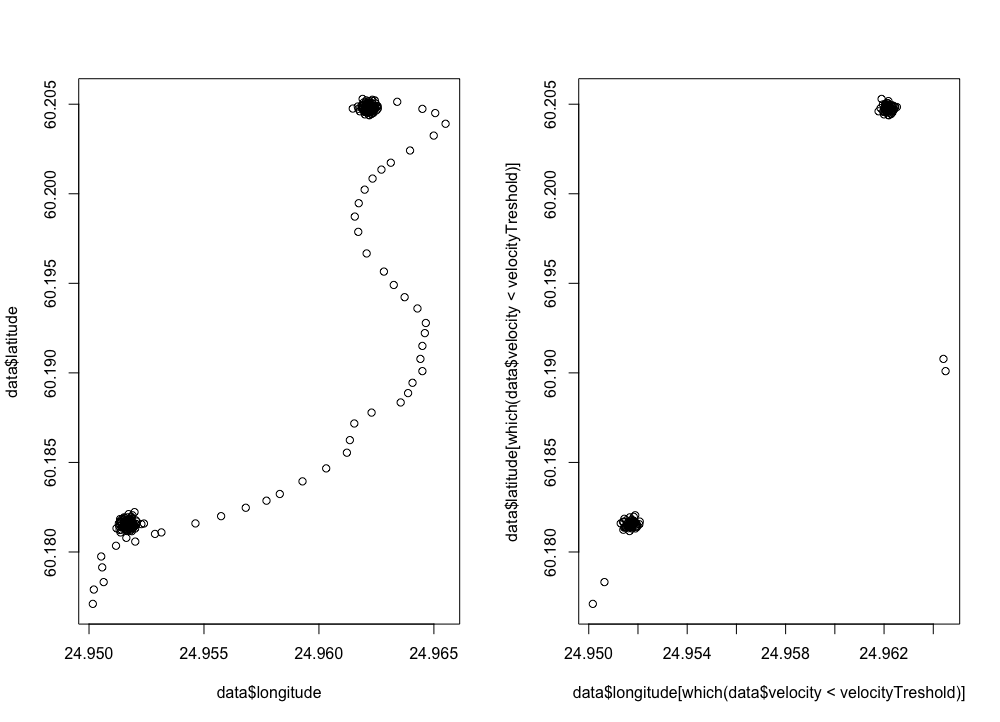
\includegraphics[width=0.75\textwidth]{images/velocity_pruning.png}
				\caption{The scatter plot of the points before (left) and after (right) the velocity pruning.}
				\label{velocity_pruning}
			\end{center}
		\end{figure}
	\item The $q$ value in the Markov chain refers to the order/memory of the model. The probability of state $x_k$ is given by the probability $p(x_k | x_{1:k-1})=p(x_k | x_{k-q-1:k-1})$	, where $x_k$ is the state of the system at time $k$, $q$ is the order of the model. In other words this means, to estimate the probability $k^{th}$ system state, $q$ number of previous observations observations are utilized. Accordingly, the first order Markov model relies only on the last observation, while a model of the $q^{th}$ order would extend the estimations with previously collected data.
		
		\item The probability transition matrices are displayed in Table \ref{probability_matrices}. The result is generated by the attached $markov\_chain.R$ script. If the user is located at Shop, the most likely place to visit next for $q=1$ is Work (50 \% chance), for $q=2$ the most likely place in order is Home (note: I was not sure how to read the probabilities in this case and therefore I looked at the corresponding lines in the table before normalizing the values and selected the place where the sum of occurrences was the highest). 
		
		To tell the most likely place in the case when the user visits Work before the Shop, the transition matrices have to be recalculated. In this case, for $q=1$ the next place is expected to be Work (55 \% chance), for $q=2$, the most likely place is Shop (50 \% chance).
		\begin{table}[]
		\centering
		\caption{The probability transition matrices of Markov Models of order one and order two for item c). }
		\label{probability_matrices}
			\begin{tabular}{rrrr}
 				\textbf{q = 1} & Home & Work & Shop \\ 
  				\hline
					Home & 0.00 & 0.64 & 0.36 \\ 
 					Work & 0.50 & 0.00 & 0.50 \\ 
  					Shop & 0.40 & 0.50 & 0.10 \\ 
   				\hline
   				\\
   				\textbf{q = 2} & Home & Work & Shop \\ 
  				\hline
					HH & 0.00 & 0.00 & 0.00 \\ 
 					HW & 0.57 & 0.00 & 0.43 \\ 
 					HS & 0.25 & 0.75 & 0.00 \\ 
  					WH & 0.00 & 0.67 & 0.33 \\ 
  					WW & 0.00 & 0.00 & 0.00 \\ 
  					WS & 0.33 & 0.50 & 0.17 \\ 
  					SH & 0.00 & 0.50 & 0.50 \\ 
  					SW & 0.40 & 0.00 & 0.60 \\ 
  					SS & 1.00 & 0.00 & 0.00 \\ 
   				\hline
			\end{tabular}	
			\end{table}
		
	\end{enumerate}
\section{Fingerprint-Based Place Detection}
		\begin{enumerate}[a)]
			\item The calculated probabilities are displayed in Table \ref{tanimoto}. The matrix is the output of the $fingerprint\_based\_detection.R$ script file. It is clearly visible that the access point number 3 has significantly lower probabilities in comparison to the other observations. This allows the conclusion that this access point has to be further away from the others and therefore at least two distinct places can be identified from the calculations. Depending on the threshold the number of places may differ, for instance for $t=0.9$ we can identify two, for $t=0.8$ three places.
		
				\begin{table}[]
					\centering
					\caption{The results of the extended Tanimoto calculations for the given access points and observations. The top table shows the results for the a) item while the bottom table shows the result for the c) item. }
					\label{tanimoto}
					\begin{tabular}{rrrrrrrrrrr}
						a) & 1 & 2 & 3 & 4 & 5 & 6 & 7 & 8 & 9 & 10 \\ 
  						\hline
						  1 & 1.00 & 0.98 & 0.86 & 0.98 & 0.98 & 0.98 & 0.98 & 0.99 & 0.93 & 0.91 \\ 
						  2 &  & 1.00 & 0.84 & 0.99 & 0.96 & 0.98 & 0.99 & 0.99 & 0.91 & 0.90 \\ 
						  3 &  &  & 1.00 & 0.84 & 0.87 & 0.86 & 0.85 & 0.86 & 0.77 & 0.75 \\ 
						  4 &  &  &  & 1.00 & 0.96 & 0.98 & 0.99 & 0.99 & 0.92 & 0.91 \\ 
						  5 &  &  &  &  & 1.00 & 0.99 & 0.97 & 0.99 & 0.90 & 0.89 \\ 
						  6 &  &  &  &  &  & 1.00 & 0.99 & 0.99 & 0.91 & 0.90 \\ 
						  7 &  &  &  &  &  &  & 1.00 & 0.99 & 0.92 & 0.90 \\ 
						  8 &  &  &  &  &  &  &  & 1.00 & 0.93 & 0.91 \\ 
						  9 &  &  &  &  &  &  &  &  & 1.00 & 0.98 \\ 
						  10 &  &  &  &  &  &  &  &  &  & 1.00 \\ 
 	  					\hline
					\end{tabular}
					\\
					\begin{tabular}{rrrrrrrrrrr}
 					c) & 1 & 2 & 3 & 4 & 5 & 6 & 7 & 8 & 9 & 10 \\ 
 					 \hline
					1 & 1.00 & 1.00 & 1.00 & 1.00 & 1.00 & 0.86 & 1.00 & 1.00 & 0.97 & 0.90 \\ 
  					2 & & 1.00 & 1.00 & 1.00 & 1.00 & 0.86 & 1.00 & 1.00 & 0.97 & 0.90 \\ 
  					3 &  & & 1.00 & 1.00 & 1.00 & 0.86 & 1.00 & 1.00 & 0.97 & 0.90 \\ 
  					4 & &  & & 1.00 & 1.00 & 0.86 & 1.00 & 1.00 & 0.97 & 0.90 \\ 
   					5 &  & & & & 1.00 & 0.86 & 1.00 & 1.00 & 0.97 & 0.90 \\ 
   					6 & & & & & & 1.00 & 0.86 & 0.86 & 0.82 & 0.76 \\ 
   					7 & & & & & & & 1.00 & 1.00 & 0.97 & 0.90 \\ 
   					8 & & & & & & & & 1.00 & 0.97 & 0.90 \\ 
   					9 & & & & & & & & & 1.00 & 0.93 \\ 
   					10 & & & & & & & & & & 1.00 \\ 
    				\hline
				\end{tabular}
				\end{table}

				\item The response rate vector is generated by the $getResponseRateVector()$ function. One of the result response rate vectors has the elements, as follows:  $[1.0 1.0 1.0 1.0 1.0 0.5 1.0 1.0 1.0 1.0]$.
				
				\item The results of the calculations are shown in Table \ref{tanimoto} (bottom). Depending on the threshold the number of places may differ, for instance for $t=0.9$ we can identify three, for $t=0.8$ four places.
			\end{enumerate}	
			

\section{Lempel-Ziv}
	
	\begin{center}
	\begin{tabular}{rrr}
		Sequence & String \\ 
  		\hline
  		$S_0 = Y$ & BANANABANDAGEBANANA \\
		$S_1 =  B$ & ANANABANDAGEBANANA \\
		$S_2 = A$ & NANABANDAGEBANANA \\
		$S_3 = N$ & ANABANDAGEBANANA \\
		$S_4 = AN$ & ABANDAGEBANANA \\
		$S_5 = AB$ & ANDAGEBANANA \\
		$S_6 = AND$ & AGEBANANA \\
		$S_7 = AG$ & EBANANA\\
		$S_8 = E$ & BANANA \\
		$S_9 = BA$ & NANA \\
		$S_{10} = NA$ & NA \\
		$S_{11} = NA$ &  \\
		\hline
	\end{tabular}
	
	\begin{figure}[h]
				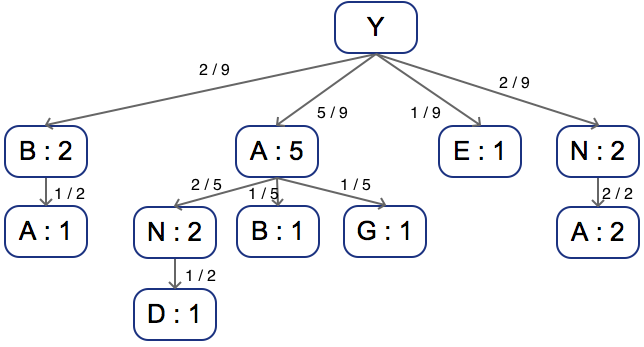
\includegraphics[width=0.75\textwidth]{images/lz-tree.png}
				\caption{The constructed LZ tree and strings for the given input.}
				\label{lz-tree}
		\end{figure}
	\end{center}
	
	\begin{eqnarray*}
		P(A) = \frac{5}{9} \\
		P(N | A) = \frac{2}{5} \\
		P(D | AN) = \frac{1}{2}
	\end{eqnarray*}

\section{Spatial Analysis: Preprocessing and Place Detection}
	The attached $spatial\_analysis.R$ file performs the preprocessing on the data. The rules to process the data are, as follows: 
	\begin{enumerate}
		\item measurements where the number of satellites is less than or equal to 3, are removed,
		\item measurements where the HDOP is greater than 6.0, are removed,
		\item points, which have no other points in their 500 meter neighborhood are considered as outliers and therefore removed. 
	\end{enumerate}
	
	The parameters are set up and can be modified in the $preprocessData()$ function. Figure \ref{spatial_analysis_preprocessing_steps} displays the points after each step in an R plot, Figure \ref{spatial_analysis_visualization} displays the point through a KML visualization in Google Maps. The clusters with $k=2$ for item b) are displayed on Figure \ref{spatial_analysis_cluster_centers}.

	\begin{figure}[h]
				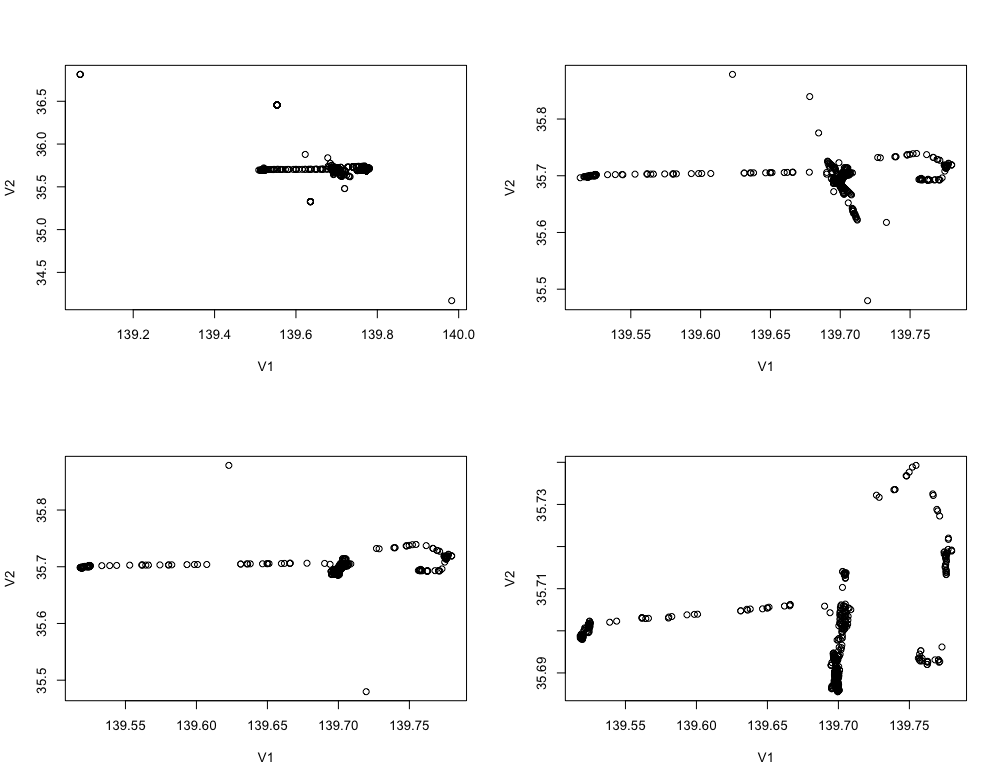
\includegraphics[width=0.75\textwidth]{images/spatial_analysis_preprocessing_steps.png}
				\caption{The data points for the Spatial Analysis task. The top left plot shows the unprocessed data set, the top right shows the points after removing points observed by 3 or less satellites, the bottom left shows the points whose HDOP value was too high and the bottom right shows the points after removing outliars. }
				\label{spatial_analysis_preprocessing_steps}
		\end{figure}
		
		\begin{figure}[h]
				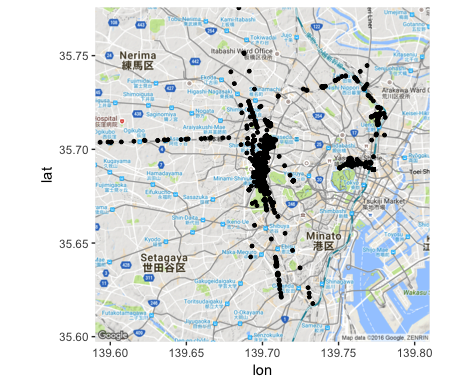
\includegraphics[width=0.75\textwidth]{images/visualized_points_before_pruning.png}
				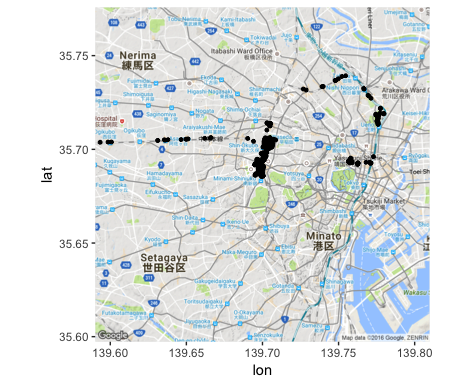
\includegraphics[width=0.75\textwidth]{images/visualized_points_after_pruning.png}
				\caption{The data points for the Spatial Analysis task visualized by KML. The top plot shows the unprocessed data set and the bottom shows the points after their pruning was performed. }
				\label{spatial_analysis_visualization}
		\end{figure}
		
		\begin{figure}[h]
				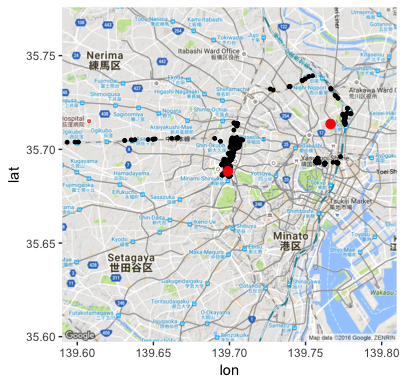
\includegraphics[width=0.75\textwidth]{images/spatial_analysis_cluster_centers.png}
				\caption{The data points (with black) and the cluster centers (with red) for the Spatial Analysis task visualized by KML.}
				\label{spatial_analysis_cluster_centers}
		\end{figure}
	
\nocite{*}
\bibliographystyle{tktl}
\bibliography{lahteet}

\lastpage

\pagestyle{empty}

\end{document}